% !TEX root = ../../thesis.tex

\chapter{Introduction} \label{introduction}

In recent decades, the rise of smart interconnected devices not only changed how we interact with information, but also introduced all-new ways of engaging with the world. The rise of smartphones enabled users to consume content and perform tasks on-the-go, tablets made people rethink the ways they work and travel and wearable devices made new sets of data available to the users. Ericsson Mobility Report of February 2021 reveals that the number of connected devices has been steadily increasing ~\cite{EricssonMobility2020}, and with new devices and form-factors underway, such as smart glasses, smart vehicles and folding displays, this trend is likely to continue in the foreseeable future. 

The increasing demand in the diversity of devices and device families also increased the demand for front-end application development, as it became more challenging and costly to have a decent user-facing online presence. This lead to advancements in front-end development; emerging new tools, techniques, frameworks, libraries, and SDKs made it possible to build consumer-facing products in ways that were never possible before. Nevertheless, the ever-growing front-end ecosystem and high user demands forced developers to spread their focus to overwhelming levels; a recent survey reveals that around \hl{TODO: This is wrong ->} 60\% of developers use more than one Front-end framework, and for cross-platform frameworks, it is more than \hl{TODO: This is wrong ->} 80\% ~\cite{StateOfJs2020} as shown in Figure ~\ref{fig:num_of_frameworks_used}. This transformation did help create a large and dynamic market of consumer products, goods and services, though it did not come without some hurdles. In this thesis, we explore what these hurdles are and discuss how Intertext addresses them.
subfigure env
\begin{figure}
  \centering
  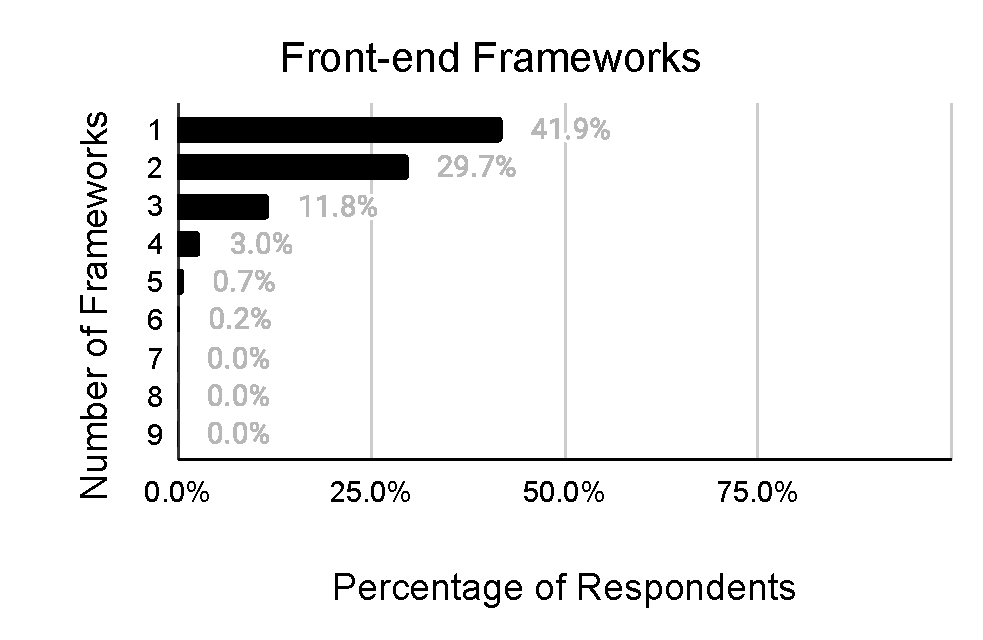
\includegraphics[width=6.2cm]{images/sojs1.pdf}
  \,
  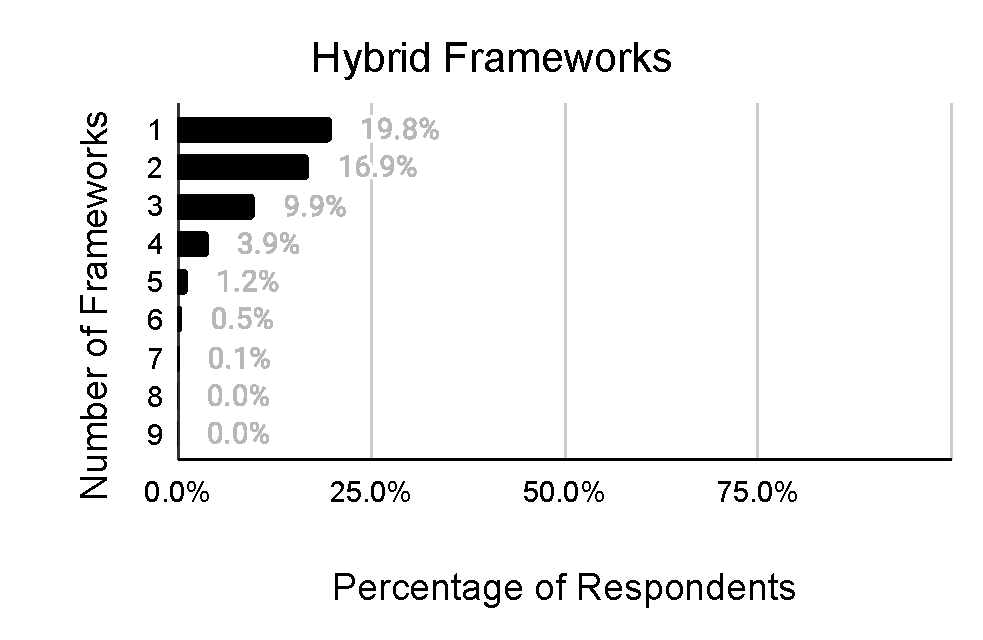
\includegraphics[width=6.2cm]{images/sojs2.pdf}
  \caption{Number of frameworks used to Percentage of respondents}%
  \label{fig:num_of_frameworks_used}%
\end{figure}

\section{Problem Statement} \label{problemStatement}

In this section, we focus on the hurdles due the increase in the diversity of devices and device families, and increasingly vibrant ecosystem of development tools and techniques. We group these hurdles in two main categories, problems faced by the end users, and problems faced by developers.

\subsection{User Problems}

The simplicity of consuming data is lost within the complexity of modern-day applications; nowadays, something as simple as checking the weather, reading a news article, browsing an image gallery, buying a product or service and filling out a form can be frustrating and time-consuming. We have identified the fundamental problems that lead to user experience problems and compromise privacy/security.

\subsubsection{UI/UX Inconsistencies}
One reason for this is the inconsistencies in front-end implementations. The visual presentation of components with the same functionality can often differ across front-end implementations, often confusing the end users. Inconsistencies are often seen not only within a platform or cross-platform, but even a single front-end application can have inconsistencies within itself. This can arise from a variety of different reasons ranging from poor design to poor implementation.

\subsubsection{Intrusive Advertisement}
Another common source of frustration for the users is intrusive online advertisement and numerous other attention-grabbing call-to-action popups that diverts users attention from the content they are consuming. A recent study by Yahoo \cite{IntrusiveAds} states that as online advertisement became the primary source of income for most products, it has become increasingly intrusive and annoying even at the cost of hurting the user experience.

\subsubsection{Lack of Accessibility}
Due to its high costs of implementation and maintenance, accessibility is often overlooked by developers. A study reveals that on an average web page, only 3.89\% of the HTML elements were found to be fully accessible \cite{WebNotForAll}. This paints a picture of how accessibility is a common problem among users.

\subsubsection{Lack of Customisability}
For many front-end applications, customisability is rarely a concern. The way of front-end ecosystem is, the developer decides on the look and feel of an application rather than the user. Although a recent trend in web design, dark mode support in front-end design \cite{DarkMode} could be seen as a shift towards more customisability. However, very few front-end applications provide such features.

\subsubsection{Lack of Cross-Platform Support}
Every now and then, we find ourselves in situations where we are trying to operate a web application with no responsiveness or touch support from our phone—or having to stand up from in front of our computer to reach for our phone because the messaging application we want to use is only available for web/desktop. Hardships in cross-platform application development often result in poor user experience due to compatibility issues and sometimes complete lack of availability.

\subsubsection{Privacy and Security Concerns}
In the open market, where everyone can create user-facing applications, there is little to no enforcement mechanism or quality control measures. At times, this results in a compromise in users security and privacy. Users, especially of old age, can be lead to downloading and executing harmful software. Without alerting the user, a foreign script can be executed on the users' computer/browser, leading to severe security and privacy concerns. 


\subsection{Developer Problems}

The complexity of building a decent, well designed, accessible front-end experience, not even once but once per every client built for various platforms, forces developers to choose between supporting multiple devices, following best practices, creating a good experience.

\subsubsection{Challenges in Development}
\begin{enumerate}
  \item Cross-platform support:
  Cross-platform application development is a prominent topic even to this day. Even though several development techniques exists \cite{PWAs}, building applications capable of running on multiple platforms is still a complex engineering challenge, and creating and maintaining multiple applications for different platforms is costly. 
  \item Accessibility support:
  Creating fully accessible applications is not always the priority for many development projects due to its costs and efforts. Accessibility implementations are often complicated as there are many different ways of creating accessible user interfaces for many different kinds of accessibility needs. A study shows that accessibility and complexity of web applications are reversely proportional, hinting that making a web page accessible hinders maintainability \cite{WebNotForAll}.
\end{enumerate}

\subsubsection{Challenges in Maintenance and Enhancements}
Building a front-end application is a great effort, but maintaining and enhancing it over time could be even more troublesome. The world of front-end development is a fast-growing and evolving ecosystem. The changes are persistent, and at times breaking. There are thousands of tools, libraries, frameworks, SDKs available at the fingertips of developers at no cost. It is a common practice to make use of these libraries as they help with the development significantly. However, the diversity in the libraries used to build the software results in a diversity of maintenance problems. Even the most well-tested and maintained libraries could break after an update, causing a headache for the developers and hardship for the users.


\section{Research Questions} \label{researchQuestions}

We have listed the problems that we are interested to solve in the section above. In light of these problems, we aim to answer the following questions in our research:

\paragraph{How can we re-imagine front-end, and improve it in such a way that:}
\begin{enumerate}
  \item from the \underline{users perspective} it:
  \begin{enumerate}
    \item presents a consistent User Experience (UX) ?
    \item works consistently on all supported devices and platforms ?
    \item allow users to customise the look and feel ?
    \item guarantees accessibility ?
    \item guarantees security and privacy ?
  \end{enumerate}
  \item from the \underline{developers perspective}, it:
  \begin{enumerate}
    \item eliminates the need to create accessible front-end applications ?
    \item eliminates the need to create front-end applications for every device/platform ?
    \item minimises the need to maintain front-end applications ?
    \item brings product development costs to a minimum?
    
  \end{enumerate}
\end{enumerate}

\section{Contributions} \label{contributions}

As discussed in the \nameref{problemStatement} (\ref{problemStatement}) section, Intertext ambitiously attempts to solve many different problems from various domains. A solution at this scale requires novelty, rethinking the current state of art instead of an incremental update. The biggest contribution of Intertext is to borrow existing concepts that are mostly academic, combine them in new ways, and apply them to solve these real-world problems. With that said, here are some notable contributions:

\begin{itemize}
  \item We reviewed existing research on User Interface Description Languages (UIDLs) and other similar topics to outline ways to utilise these concepts to solve the aforementioned problems.
  \item We designed IUIDL and while doing so, we decided:
  \begin{itemize}
    \item What are the concepts that are crucial to modern front-end development that needs support out-of-the-box
    \item What terminology should we use in order to create an optimal balance between the device-independent nature and developer familiarity
    \item What the syntax should be like to maximise developer friendliness
    \item How to overcome some limitation of XML in the most effective, clear and extendable way
  \end{itemize}
  \item We created an engine using JavaScript/Typescript to perform common tasks of Intertext clients, such as parsing IUIDL and managing the application state
  \item We created multiple software clients that can render IUIDL into functional front-ends optimised for the host device and are user customisable where possible
\end{itemize}


\section{Methodology} \label{methodology}

To identify and effectively address all these problems, we utilised the Design Science Research Methodology (DSRM) \cite{DSRM} to carry out our research. DSRM is a commonly adopted research framework that provides six executable steps to guide the researcher in being consistent with prior work and provides a theoretical process for doing the research, and guides through presenting and evaluating the outcome. 

The first step of DSRM is \textbf{identifying the problem and the motivation}. It is not uncommon for research and inventions to stem from a problem or a necessity. Similarly, in our case, the problem was out there; we only needed to focus on it to better understand the issues we are tackling. In \nameref{problemStatement}, we discussed and justified what problems we are attempting to solve with Intertext. Then we proceeded to the next step, \textbf{defining the objectives for a solution}. As we narrowed down the problems that we attempt to solve in \nameref{problemStatement}, we drafted our objectives to approach this problem. We explained these objectives in detail in \nameref{researchQuestions}. Then, we were ready to take the next step of \textbf{design and development}. In the sections \nameref{solution} and \nameref{implementation}, we explained in detail our development process, all the challenges and design decisions that we have taken in order to address the problems in the best way possible. 

Once we had a working prototype, we created a simple Intertext application, RecipeApp, as explained in detail in \nameref{evaluation} section. This application served as a demonstration for developers on how IUIDL could be dynamically served from a backend. We also introduced Intertext to end users, communicated its goals and motivations, and then collected feedback. These concludes the final three steps of \textbf{demonstration}, \textbf{evaluation} and \textbf{communication} into one.

\section{Structure} \label{structure}

\begin{enumerate}
    
    \item \textbf{\nameref{relatedWork}}: In this section, we first explore similar research that has been done. We evaluate several of the UIDLs, discuss the similarities and what separates Intertext from them. We also introduce other libraries, frameworks, tools, services and other solutions similar to Intertext.

    \item \textbf{\nameref{solution}}: In this section, we thoroughly discuss the details of the Intertext project. We first walk through the design principles and explain the purpose behind each, and what problems in the \nameref{problemStatement} are they aiming to address. Then, we introduce Intertext User Interface Description Language (IUIDL), our XML-based markup language. Finally, we talk about Intertext clients, what they are, and how they work.

    \item \textbf{\nameref{implementation}}: This section talks about the overall architecture of Intertext. We first talk about Intertext engine and several other core components of Intertext. Then, we list the Components and Commands that IUIDL offers out of the box.
    
    \item \textbf{\nameref{evaluation}}: In this section we give example use-cases scenarios for the users, and walk through the sample RecipeApp that intends to serve as an example use-case for developers in technical sense. Then, we move on the user evaluation; first we explain our methodology, and then we share the results.

    \item \textbf{\nameref{discussion}}: In this section, we explain how we addressed the problems in \nameref{problemStatement} and how we answer the questions in \nameref{researchQuestions}. Then, we talk about the limitations.

    \item \textbf{\nameref{conclusion}}: In this section we list our main contributions with Intertext project, and give a non-exclusive list of our future plans.
    
\end{enumerate}